\documentclass[a4paper,11pt]{article}
\usepackage[margin=22mm]{geometry}
\usepackage{fontspec,amsmath,booktabs,graphicx,hyperref}
\setmainfont{STIXGeneral}\setlength{\emergencystretch}{2em}
\begin{document}
\begin{center}{\Large Topic D: proofs and their costs}\\[4pt]Human Compression project\end{center}
The common paper on stabilizers, support and enumeration supports three complete
applications: commuting involutions (D1), Suzuki polyhedra (D2), and Hall--Janko
geometries (D3). The comparison preserves the thirty-seven admitted source clauses
and their stated qualifications. The paired graph records actual proof routes;
it does not replace the complete manuscripts by their shortest selected routes.

\paragraph{Written papers.}
The three complete source PDFs cost 47,894 characters. The whole common theory
costs 15,632 and the three applications cost 29,855, giving
\[R_D^{\mathrm{written}}=\frac{47\,894}{15\,632+29\,855}
 =\frac{47\,894}{45\,487}=1.052916\ldots.\]
Title, abstract, definitions, proofs, tables, context and references are included.
The unused normalizer theorem remains paid as part of the whole common paper.

\paragraph{Including the complete program.}
The twelve-page appendix preserves five required mathematical programs and
three complete diagnostics. All eight are charged, including comments and the
wrapper, at 27,070 characters. The separate comparison is
\[R_D^{\mathrm{programs}}=\frac{47\,894}{45\,487+27\,070}
 =\frac{47\,894}{72\,557}=0.660088\ldots.\]
The full eight raw files cost 26,185; substituting them for the printed appendix
gives $47\,894/71\,672=0.668239\ldots$. They are alternatives, never additional
charges. Two complete operational drivers cost 10,038 raw characters and
12,765 actual bytes, separately inventoried rather than included in these factors.

\begin{center}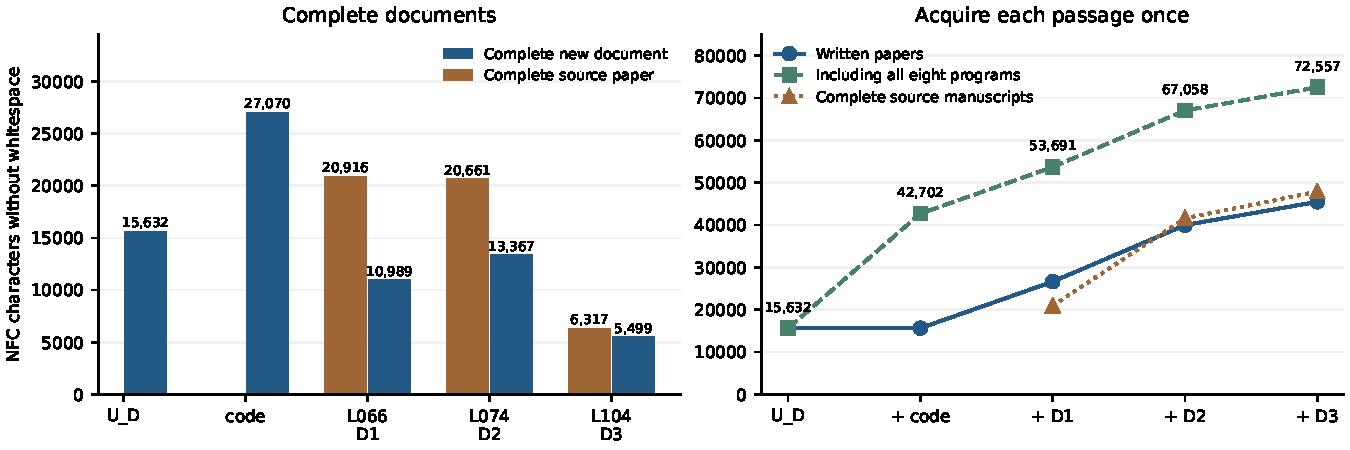
\includegraphics[width=\linewidth]{acquisition.pdf}\end{center}
\noindent These figures use calibrated complete PDF extracted text, NFC characters
without whitespace. All thirty policy coordinates are provided. Expanded external
proofs, catalogue and algorithm construction, historical software, and graphics
remain unknown costs, not zero.

\paragraph{After acquiring the whole common theory and all eight programs.}
\begin{center}\begin{tabular}{lrrr}\toprule
Source / application & Complete source & Complete application & Conditional factor\\\midrule
L066 / D1 & 20,916 & 10,989 & 1.903\\
L074 / D2 & 20,661 & 13,367 & 1.546\\
L104 / D3 & 6,317 & 5,499 & 1.149\\
\bottomrule\end{tabular}\end{center}
\newpage
\paragraph{Acquisition and reuse.}
Acquire the whole $U_D$, the complete program appendix, and then D1, D2 and D3.
For the union $K_i$ of passage owners paid through stage $i$, the new cost is
$c(K_i\setminus K_{i-1})$. Every application is charged in full. Previously
acquired prerequisites are not charged again, and no common theory is discounted
because another topic uses overlapping arguments.
\begin{center}\begin{tabular}{lrrrr}\toprule
Added & New cost & Written total & With programs & Prior text used\\\midrule
U\_D & 15,632 & 15,632 & 15,632 & ---\\
CODE & 27,070 & 15,632 & 42,702 & ---\\
D1 & 10,989 & 26,621 & 53,691 & 8,446\\
D2 & 13,367 & 39,988 & 67,058 & 3,222\\
D3 & 5,499 & 45,487 & 72,557 & 21,663\\
\bottomrule\end{tabular}\end{center}
The last column is the owner union of already acquired text used by the local
paper's recorded arguments. It is not a further subtraction from the application's
length. The matching historical cumulative costs are 20,916, 41,577 and 47,894.
This is a declared reading order, not a research chronology or a claim of a
sawtooth pattern.

\paragraph{What a proof route measures.}
Each of the 37 clauses has a historical route and a current proof or explicit
retention/exclusion boundary. The generating-series and faithfulness outputs are
shown separately, without new source credit. For a set of prerequisite nodes
$S$, its known text cost is
\[c_{\mathrm{route}}(S)=c\!\left(\bigcup_{v\in S}\operatorname{owners}(v)\right).\]
Historical arrows document the reasoning asserted in each source; they do not
retroactively certify a corrected or overbroad historical lemma.
Shared statement passages and program wrappers therefore appear once in a union.
Repeated physically printed statements remain counted at every location.
Context outside a selected route remains paid in the complete-paper comparisons.
No factor is computed from a route subtotal, box sum or number of nodes.

The logical graph has 137 nodes and 284 typed arrows: 50 historical nodes,
58 current nodes, 20 external inputs and 9 verification components. The cost
partition has 220 owners and 215 selected-text spans. Every extracted character
belongs to exactly one owner in each of the three text policies. The untrimmed
sensitivity assigns furniture to explicit owners. Both Unicode normalizations
and all five counting units conserve every whole-document total.

\paragraph{Scope and evidence.}
L066's corrected reversal argument and exceptional full-automorphism computation
remain distinct from its historical proof. The Suzuki local normalization,
generation, intersection and duality checks are paid alongside the common
support count; Suzuki's classification, Lüneburg's structure and other classical
inputs retain their original attribution and unknown expanded costs.
The Hall--Janko census includes every Borel anchor and the complete geometric
recognition tests. Its printed diagrams, full geometric automorphism/correlation
groups, doubling relation and supplement annotations remain excluded from the
fixed principal census contract. Their source text is still charged.

The five required programs enter logical routes; the three diagnostics have
positive printed costs but only validation arrows. The original ten scoped Lean
declarations and the later generic supplement of 28 declarations are formal
evidence, not complete formalizations of the applications. The latter comprises
12 plus 16 declarations, not 12 in addition to 28.

The input calibration uses the accepted occurrence-bound repairs, including the
L066 extracted-character/encoding collision; that embedded font has no
ToUnicode stream. No source PDF, primary text or source raster is exported.
The offline viewer exposes proof locations, actual edges, owners and unknown
inputs. Its deterministic DOM tests are not real-browser layout tests. This
ownership and reader packet awaits independent review and changes no accepted
paper factor, source credit or question credit.
\end{document}
